\documentclass[10pt, a4paper,UTF8]{article}
\usepackage{graphicx}
\usepackage{ctex}
\usepackage{CJK}
\usepackage{amsmath}
\usepackage{makecell}%表格竖线连续
\newcommand\toprule{\Xhline{.08em}}
\newcommand\midrule{\Xhline{.05em}}
\newcommand\bottomrule{\Xhline{.08em}}
\def\I{\vrule width1.2pt}
%!\I 就可以代替| 来画表格了

%可固定下划线长度
\makeatletter
\newcommand\dlmu[2][4cm]{\hskip1pt\underline{\hb@xt@ #1{\hss#2\hss}}\hskip3pt}
\makeatother


\usepackage{array}%数学
\usepackage{multirow}%跨行表格
%\usepackage[colorlinks,linkcolor=red]{hyperref}%超链接

\usepackage{fancyhdr}  %使用fancyhdr包自定义页眉页脚
%\pagestyle{empty}
\pagestyle{fancy}
%\pagestyle{plain}%没有页眉,页脚放页数
\renewcommand{\headrulewidth}{0.5pt}
\renewcommand{\footrulewidth}{0.4pt}
\lhead{}
\chead{}
\rhead{}
\lfoot{}
\cfoot{\thepage}
\rfoot{}


\usepackage{booktabs}%表格用

\usepackage{float}%可以用于禁止浮动体浮动

%目录超链接
\usepackage[colorlinks,linkcolor=black,anchorcolor=blue,citecolor=black]{hyperref}

\usepackage{listings}%可以插入代码
\usepackage{xcolor}%语法高亮支持
%代码格式
\definecolor{dkgreen}{rgb}{0,0.6,0}
\definecolor{gray}{rgb}{0.5,0.5,0.5}
\definecolor{mauve}{rgb}{0.58,0,0.82}
\lstset{ %
	language=Matlab,                % the language of the code
	breaklines,%自动折行
	%extendedchars=false%解决代码跨页时,章节标题,页眉等汉字不显示的问题
	keepspaces=false,  
	%tabsize=4 %设置tab空格数
	showspaces=false,  %不显示空格
	showtabs=false,  
	showstringspaces=true, 
	numbers=left, 
	basicstyle=\footnotesize, 
	numberstyle=\tiny, 
	numbersep=5pt, 
	keywordstyle= \color{ blue!70},%关键字颜色
	commentstyle= \color{red!50!green!50!blue!50},%注释颜色 
	frame=shadowbox, % 边框格式:阴影效果
	rulesepcolor= \color{ red!20!green!20!blue!20} ,
	escapeinside=``, % 英文分号中可写入中文
	xleftmargin=2em,xrightmargin=2em, aboveskip=1em,%设置页边距
	framexleftmargin=2em
}




%设置页面格式
\usepackage[left=2.0cm, right=2.0cm, top=2.0cm, bottom=2.0cm]{geometry}

\begin{document}

%%%%%%%%%%%%%%%%%%%%%%%%%%%%%%
%% 封面部分
%%%%%%%%%%%%%%%%%%%%%%%%%%%%%%
\begin{titlepage}
	\begin{minipage}[c]{0.75\textwidth}
		\centering
		
\includegraphics[width=0.5\textwidth]{logo.jpg}
		%{\LARGE 软件学院}
	\end{minipage}
\vspace{0.5cm}	
\centering

{\Huge\kaishu{\quad Optimization Method Homework1\par}}


\vspace{7cm}

\begin{flushleft}

{\fangsong\Large \qquad\qquad\qquad\qquad 姓\qquad 名:\dlmu[8cm]{丁毅}\par}
\vspace{.1cm}
{\fangsong\Large \qquad\qquad\qquad\qquad 专\qquad 业:\dlmu[8cm]{电信学部 硕9065班}\par}
\vspace{.1cm}
{\fangsong\Large \qquad\qquad\qquad\qquad 学\qquad 号:\dlmu[8cm]{3119105343}\par}
\vspace{.1cm}
{\fangsong\Large \qquad\qquad\qquad\qquad 联系方式:\dlmu[8cm]{1048585782@qq.com}\par}
\end{flushleft}
% Table generated by Excel2LaTeX from sheet 'Sheet1'
% Table generated by Excel2LaTeX from sheet 'Sheet1'


\end{titlepage}
\newpage

\section{问题描述}
使用共轭梯度法求解高阶二次函数。共轭梯度法(Conjugate Gradient)是介于最速下降法与牛顿法之间的一个方法,它仅需利用一阶导数信息,但克服了最速下降法收敛慢的缺点,又避免了牛顿法需要存储和计算Hesse矩阵并求逆的缺点,共轭梯度法不仅是解决大型线性方程组最有用的方法之一,也是解大型非线性最优化最有效的算法之一。 在各种优化算法中,共轭梯度法是非常重要的一种。其优点是所需存储量小,具有步收敛性,稳定性高,而且不需要任何外来参数。
\paragraph{}
使用共轭梯度法求解方程
\begin{equation}
    f(x_1, x_2) = 2x_{1}^2 + x_{2}^2 - 2x_{1}x_{2} - 4x_{2}
\end{equation}
的极小点和极小值。

\section{求解}
解:设定初始点为$[1, 1]^T$, 迭代精度为$\epsilon=0.001$
\par
\qquad 1)第一次沿负梯度方向进行搜索
\par
\qquad 计算初始点的梯度:
$$ \nabla f\left(\boldsymbol{x}^{0}\right)=\left[\begin{array}{c}{4 x_{1}-2 x_{2}} \\ {2 x_{2}-2 x_{1} - 4}\end{array}\right]_{x^{0}}=\left[\begin{array}{c}{2} \\ {-4}\end{array}\right] $$

$$ x^{1}=x^{0}+\alpha_{0} d^{0}=\left[\begin{array}{l}{1} \\ {1}\end{array}\right]+\alpha_{0}\left[\begin{array}{c}{2} \\ {-4}\end{array}\right]=\left[\begin{array}{c}{1+2 \alpha_{0}} \\ {1-4 \alpha_{0}}\end{array}\right] $$

\qquad 一维最佳搜索步长应满足:

$$ f\left(x^{1}\right)=\min _{\alpha} f\left(x^{0}+\alpha d^{0}\right)=\min _{\alpha}\left(40 \alpha^{2}+20 \alpha-3\right)  $$

\par
\qquad 此时:

$$ \alpha_{0}=0.25 \quad \boldsymbol{x}^{1}=\left[\begin{array}{c}{0.5} \\ {2}\end{array}\right] \quad \nabla f\left(\boldsymbol{x}^{1}\right)=\left[\begin{array}{c}{-2} \\ {-1}\end{array}\right] $$

\par
\qquad 2)第二次迭代
$$ \beta_{0}=\frac{\left\|\nabla f\left(\boldsymbol{x}^{1}\right)\right\|^{2}}{\left\|\nabla f\left(\boldsymbol{x}^{0}\right)\right\|^{2}}=\frac{5}{20}=0.25 $$

$$ \boldsymbol{d}^{1}=-\nabla f\left(\boldsymbol{x}^{1}\right)+\beta_{0} \boldsymbol{d}^{0}=\left[\begin{array}{c}{1.5} \\ {2}\end{array}\right] $$

$$ x^{2}=x^{1}+\alpha d^{1}=\left[\begin{array}{c}{0.5} \\ {2}\end{array}\right]+\alpha\left[\begin{array}{c}{1.5} \\ {2}\end{array}\right]=\left[\begin{array}{c}{0.5+1.5 \alpha} \\ {2+2 \alpha}\end{array}\right] $$

\qquad 带入目标函数:
$$ \begin{aligned} f(x) &=2(0.5+1.5 \alpha)^{2}+(2+2 \alpha)^{2}-\\ & 2(0.5+1.5 \alpha)(2+2 \alpha)-4(2+2 \alpha)=\phi(\alpha) \end{aligned}  $$

\qquad 求解得 $\alpha = 1$
\par
\qquad 因此得:
$$ \boldsymbol{x}^{2}=\left[\begin{array}{l}{2} \\ {4}\end{array}\right], \quad f\left(\boldsymbol{x}^{2}\right)=-8, \quad \nabla f\left(\boldsymbol{x}^{2}\right)=\left[\begin{array}{l}{0} \\ {0}\end{array}\right] $$
\qquad 因为:$ \left\|\nabla f\left(\boldsymbol{x}^{2}\right)\right\|=0<\varepsilon $
\par
\qquad 迭代收敛。
\par
\qquad 因此,目标函数得极小点为 $[2, 4]^T$,极小值为$-8$。

\section{程序}

首先是共轭梯度算法函数:

\begin{lstlisting}
    function [f_v, best_x, iteration_num] = conjungate_gradient(f, x, x0, epsilon)
    %input
    % f - object functiuon
    % x - var
    % x_0 - Initial point
    % epsilon - tolerance
    
    %output
    % f_v - minimum f value
    % best_x - mimimum point
    % iteration_num - iteration count
    %% init
    syms betas
    
    n = length(x)
    
    n_f = cell(1, n)
    
    for i = 1 : n
        n_f{i} = diff(f, x{i});
    end
    
    %initial gradient
    n_fv = subs(n_f, x, x0);
    
    n_fv_pre = n_fv;
    
    
    count = 0;
    k = 0;
    x_v = x0;
    
    %initial search direction
    d = - n_fv;
    
    fprintf('Initial:\n');
    fprintf('f = %s, x0 = %s, epsilon = %f\n\n', char(f), num2str(x0), epsilon);
    
    while (norm(n_fv) > epsilon)
        x_v = x_v + betas * d;
        phi = subs(f, x, x_v);
        n_phi = diff(phi);
        beta = solve(n_phi);
        beta = double(beta);
       
        
        if beta < 1e-5
            break;
        end
        
        x_v = subs(x_v, betas, beta);
        x_v = double(x_v);
        n_fv = subs(n_f, x, x_v);
        count = count + 1;
        k = k + 1;
        alpha = sumsqr(n_fv) / sumsqr(n_fv_pre);
        
        fprintf('Iteration: %d\n', count);
        fprintf('x(%d) = %s, lambda = %f\n', count, num2str(x_v), beta);
        fprintf('nf(x) = %s, norm(nf) = %f\n', num2str(double(n_fv)), norm(double(n_fv)));
        fprintf('d = %s, alpha = %f\n', num2str(double(d)), double(alpha));
        fprintf('\n');
        
        d = - n_fv + alpha * d;
        n_fv_pre = n_fv;
        if k >= n
            k = 0;
            d = - n_fv;
        end
    end
    
    f_v = double(subs(f, x, x_v));
    best_x = double(x_v);
    iteration_num = count;
    
    end
\end{lstlisting}

使用上述函数进行测试:

\begin{lstlisting}
syms x1 x2;
f = 2 * x1^2 + x2^2 - 4*x2 - 2*x1*x2;
x = {x1, x2};

x0 = [1 1];

epsilon = 1e-8;

[bestf, bestx, count] = conjungate_gradient(f, x, x0, epsilon);
% print result
fprintf('bestx = %s, bestf = %f, count = %d\n', num2str(bestx), bestf, count);
\end{lstlisting}


\section{结果}

\begin{figure}[H]
	\centering
	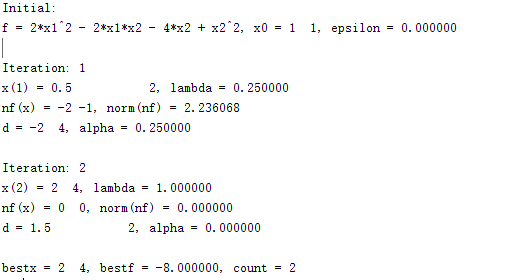
\includegraphics{rs.PNG}        %这个是在LaTeX文件夹中的相对路径
    \caption{程序运行结果1}
    \label{fig2}
\end{figure}

可以看出,程序在进行2次迭代后收敛,并且求得得结果和精确解一致。
\par
而面对更复杂的函数如:


 $$   f(x_1,x_2) = (x_1-1)^4 + (x_1 - x_2)^2 $$

 则需要更多的迭代次数才能够收敛:

 \begin{figure}[H]
	\centering
	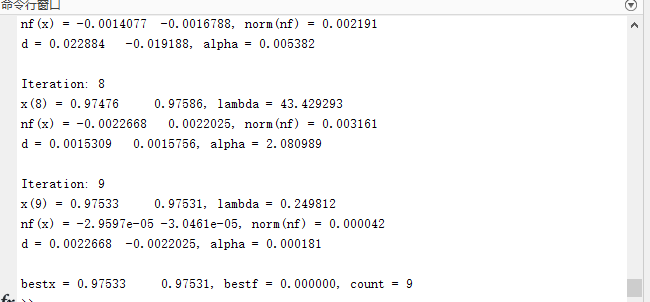
\includegraphics[scale=0.8]{rs2.PNG}        %这个是在LaTeX文件夹中的相对路径
    \caption{程序运行结果2}
    \label{fig2}
\end{figure}

\section{总结}
\begin{itemize}
    \item 由结果看出,程序经过两次迭代后就收来奶得到了结果,证明共轭梯度法收敛速度较快,计算量较小,稳定性高,一般来说,$n$维的优化问题迭代$n$次就可以收敛。
    \item 选择不同地初始点坐标,经过迭代后得到的结果是一样的,说明共轭梯度法的结果不受初始点选择的影响。
    \item 迭代精度越高时,程序的运行时间越长,迭代次数越多,因此在解决实际问题中我们需要选择一个合适的迭代精度,充分利用计算的效率。
\end{itemize}


\end{document}
